% Initiated by 정민석(2014년도 경기과학고 수학과전문교원)
% Continously being modified by 경기과학고 TeX 사용자협회
% Website : http://gshslatexintro.github.io 
\documentclass{gshs-report-v1.2}
% 추가로 필요한 패키지가 있다면 주석을 풀고 적어넣으십시오,
%\usepackage{...}

\researchtype{기초} % 기초 / 심화
\reporttype{중간} % 중간 / 결과

\title{가중치가 있는 투표자 모형: 권위자의 영향과 최적의 의사 결정 모형} % 제목 개행 시 \linebreak 사용. \\나 \newline 은 안됨.
\englishtitle{Voter model with weight : Influence of authority and optimum decision-making model}% 제목 개행 시 \linebreak 사용. \\나 \newline 은 안됨.

\author[1] {박종하} % 제 1 저자명
\email[1]{kevin0512@naver.com} % 제 1 저자 이메일
\author[2] {유광민} % 제 2 저자명
\email[2]{kyle0303@naver.com} % 제 2 저자 이메일
\author[3] {최진수} % 제 3 저자명
\email[3]{cjs33233@naver.com} % 제 3 저자 이메일
\advisor{서울} % 지도교사명
\advisorEmail{wool@wool.pe.kr} % 지도교사 이메일

%%%%%%%%%%%%%%%%%%%%%%%%%%%%%%%%%%%%%%%%%%%%%%%
%%%% researchtype이 '심화'일 경우에만 나타남 %%%%
\professor{교수님} % 지도교수명
\professorEmail{professor@e-mail.address} % 지도교수 이메일
%%%%%%%%%%%%%%%%%%%%%%%%%%%%%%%%%%%%%%%%%%%%%%%%
\summitdate{2016}{06}{12} % 제출일 (연, 월, 일)
\newtheorem{definition}{정의}


% 아래의 함수를 사용하면 이미지 파일들을 같은 디렉토리 내에 images 라는 이름을 가진 폴더를 생성한 후, 그 폴더 안에 넣어 사용할 수 있습니다.
% 사용하고자 한다면 주석을 푸십시오.
%\graphicspath{{images/}}

% 아래와 같은 command를 만들면 길이가 긴 용어를 간편하게 사용할 수 있습니다. 단, 이미 지정된 함수명들은 새로운 함수명으로 사용할 수 없습니다.
\newcommand{\gshs}{Gyeonggi Science High School }

% 본문 시작
\begin{document}

%표지만들기
%makecover 함수와 관련하여 "Underfull \hbox (badness 10000) in paragraph" 오류는 무시하십시오. (TeXstudio ver 2.9.4 오류 기준)
\makecover

%초록(영문)

%\begin{abstract}
%\noindent{
%	Put your abstract here. Once upon a time, \gshs said : `The first, and the best.'
%}
%\end{abstract}

%초록(한글)
\begin{abstractkor}
\noindent{
	본 연구 내용에서 실행한 기존의 몬테카를로 시뮬레이션을 통해 몬테카를로 시뮬레이션을 앞으로의 연구에 사용할 수 있게 되었다. 또한, voter model을 이용한 시뮬레이션 결과를 통해 군대형 구조에서 최고 권위자가 잘못된 결정을 하면 집단 전체가 빠른 시간안에 잘못된 결론을 낸다는 것을 확인했다.
}
\end{abstractkor}


\section{Introduction}
최근 통계물리학자들은 통계물리학의 이론을 기존 물리학의 범위에만 적용하지 않고 생물, 의학, 정보과학을 비롯한 다른 분야에도 적용하고 있다. 이는 기존의 물리 현상은 현대 물리학으로 잘 설명이 되고 있고 통계물리학 이론이 다른 분야에서도 굉장히 잘 들어맞기 때문이다. \cite{Stauffer06} 특히 사회학에 적용하는 시도 또한 성공적으로 진행되고 있는데, 이는 인간 개개인이 집합을 구성하는 작은 입자에 대응되고, 인간간의 상호작용이 작은 입자간의 역학적 상호작용과 매우 유사한 모습을 보이기 때문이다.\cite{Stauffer08} 
통계학을 이용하여 설명한 다양한 사회현상이 있는데, 대표적으로 ‘Opinion dynamics’가 있다. 의사결정은 그룹 안에서의 상호작용 중 가장 중요한 요소인데, 이 것을 연구하는 것이 ‘Opinion dynamics’이다.\cite{Hegselmann02} ‘Opinion dynamics’에는 다양한 모델이 있는데 대표적으로 투표자 모형이 있다. 투표자 모형은 복잡한 구조에서 연속적인 입자간의 역학적 상호작용이 일어나는 모델이다. 이 투표자 모형은 사회 현상을 설명하기 아주 효과적이다.\cite{Han10} 본 연구의 선행연구는 투표자 모형을 사용하여 민주적인 집단의 의사 결정이 더 합리적이라는 것을 시뮬레이션을 통해 증명했다. 이 논문에서 설정한 모델은 민주주의가 더 합리적이라는 것을 증명하기에는 효과적 이였지만 실제 사회와는 조금 다르다. 이 논문에서는 다른 사람들과 의견을 주고받을 때 자신의 의견이 바뀔 확률이 항상 일정하다고 했는데 실제 사회에서는 상호작용하는 대상에 따라 의견이 바뀔 확률이 다르다. 본 연구에서는 기존의 통계 물리학 시뮬레이션과 선행 연구들의 시뮬레이션 과정을 재현한 후, 사회에서의 권위 또는 영향력과 대응되는 가중치를 각각의 입자에 적용한 투표자 모형을 설계하고 시뮬레이션을 진행해 권위와 영향력이 의사 결정에 미치는 영향을 분석한 다음, 이를 토대로 가장 효율적인 의사 결정 구조를 만들 것이다.



%-----------------------------------------------------
% Next Section (e.g. Experiment, Linear theory, etc...) 
%-----------------------------------------------------
\section{Theoretical background}
통계 물리학 연구의 기본이 되는 몬테카를로 시뮬레이션과 사회에 적용한 다양한 모델 중 본 연구에서 이용할 Voter model과 Ising model에 대해 알아본다.

\subsection{Monte Carlo simulation}

난수(정의된 범위 내에서 무작위로 추출된 수)를 이용하여 함수의 값을 확률적으로 계산하는 알고리즘을 말한다. 난수를 함수에서 수많이 호출하여서 각각의 함수 값을 구하고, 이를 이용하여 확률을 계산한다. 난수를 많이 호출할수록 확률은 더욱 정확해진다. 확실한 수학적 계산으로 구하기 어렵거나 불가능한 확률을 계산하는데 유용하게 사용된다. 
몬테카를로 시뮬레이션을 이용하는 예시로는 원주율 π구하기를 들 수 있다. 

\begin{itemize}
	\item{한 변의 길이가 2r인 정사각형을 그린다.(넓이 $4r^2$)}
	\item{정사각형에 내접하는 반지름 r인 원을 그린다.(넓이π$r^2$)}
	\item{정사각형 내부에 무작위로 점을 찍는다. }
	\item{원 내부의 점과 찍은점의 수를 구한다.(점의 수가 많이 질수록 점의 수는 넓이와 비례)}
	\item{원의 넓이/정사각형의 넓이 = π$r^2/4r^2$ = π$/4$}
	\item{π를 구한다.}
\end{itemize}
원래 π를 구하는 방식대로라면 복잡한 수식을 계산해야 한다. 그 방법 대신 이러한 방법으로도 원주율을 구할 수 있다.


\subsection{Voter model}

voter model의 정의는 매우 간단하다. 각각의 개체는 s=+1 또는 -1의 값을 가질 수 있다. 매 단계에서 임의의 개체 i를 선택하고 i와 이웃해 있는 개체 중 임의의 개체 j를 선택하면 si = sj 즉, 임의의 개체는 그의 이웃 개체의 의견을 수용한다. Ising model의 자기스핀과 voter model의 s와 대응시킬 수 있으며 voter model의 상호작용 또한 zero-temperature Glauber dynamic을 Ising model에 적용한 것과 유사하다. 이러한 유사성을 이용해서 구한 \cite{Frachebourg96} d차원에서의 voter model에서 si가 –si로 바뀔 확률 Wi(s)는 다음과 같다.

\begin{equation}
\ {W}_i(s)=d/4(1-s_i/2d\sum_j\ {s}_j)\nonumber
\end{equation}

또한 이웃한 두 개체의 의견이 다른 정도를 뜻하는 n는 d에 따라 다음과 같이 달라진다.
\begin{align}
\ (d<2):n(t)= t^{-(2-d)/2}	\\
\ (d=2):n(t)= 1/ln(t)	\\
\ (d>2):n(t)= a-bt^{-d/2}
\end{align}

d가 2 이하일 경우 n가 0으로 수렴하고 2 초과일 경우 아무리 오랜 시간이 지나도 0이 되지 않는다. 즉, d가 2이하일 경우에만 개체 전체 집단의 의견 일치가 일어난다는 것이다. 이러한 상호작용에서 공통적인 특징이 나타나는데, 무작위적으로 결정된 의견이 상호작용이 일어남에 따라 전체 계가 준안정적인 상태가 되는데 이 상태가 진행되는 시간 τ가 길수록 전체 계의 n가 0에 수렴한다. 또한, 전체 계의 개체수 N이 증가할수록 τ가 증가한다.\cite{Han10}
%-----------------------------------------------------
% Conclusion
%-----------------------------------------------------

\section{연구 내용}

본 연구를 진행하기 전에, 위에서 알아본 이론적 배경을 바탕으로 기존의 몬테카를로 시뮬레이션과 Voter model on a directed network: Role of bidirectional opinion exchanges\cite{Han10}의 연구 과정을 재현해 보았다.

\subsection{Monte Carlo simultaion}

우리는 몬테카를로 시뮬레이션을 이해하여 연구에 이용하기 위해 난수 설정과 몬테카를로 시뮬레이션을 직접 수행해 보았다.
첫 번째로 난수의 설정을 연습해 보았다.

\begin{figure}[h]
	\begin{center}
		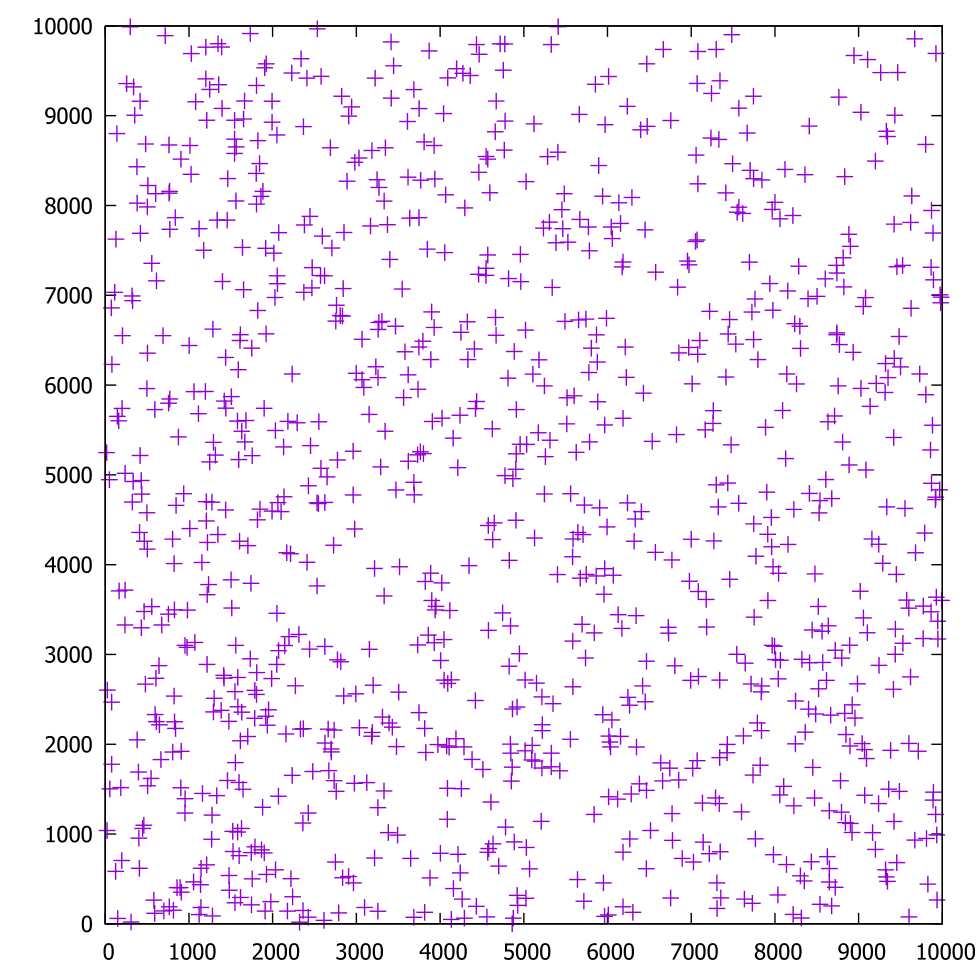
\includegraphics[width=5cm]{x,y simul2 1000.png}\\
		\caption{$10^4*10^4$의 x y 평면에 1000개의 점을 무작위로 분포시켜 보았다. 특정한 어느 좌표에 점이 몰리지 않고 상당히 균등하게 배치된 것을 알 수 있다.} 
		\label{Fig01}
	\end{center}
\end{figure}
\begin{figure}[h]
	\begin{center}
		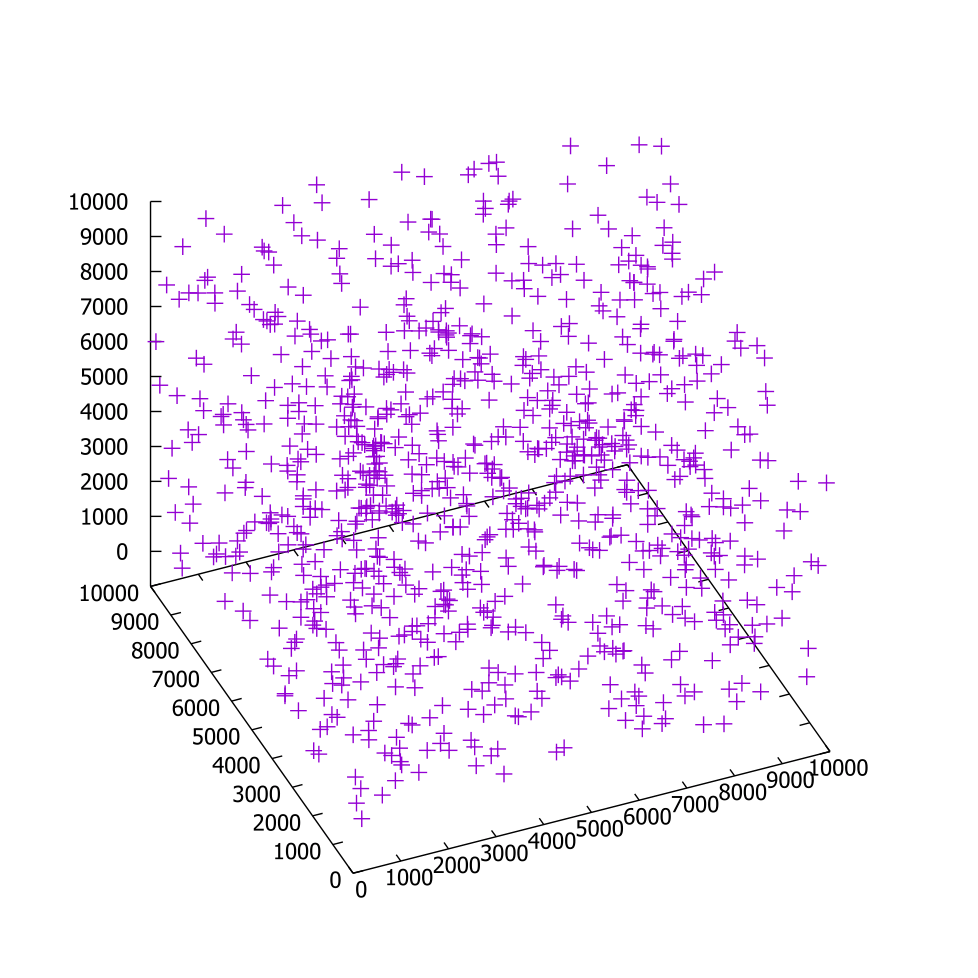
\includegraphics[width=5cm]{x,y,z simul.png}\\
		\caption{$10^4*10^4*10^4$의 x y z 공간도 마찬가지 이다. 2000개의 점을 찍어서 비교를 해보니 고르게 분포한 것을 알 수 있다.} 
		\label{Fig02}
	\end{center}
\end{figure}
\begin{figure}[t]
	\begin{center}
		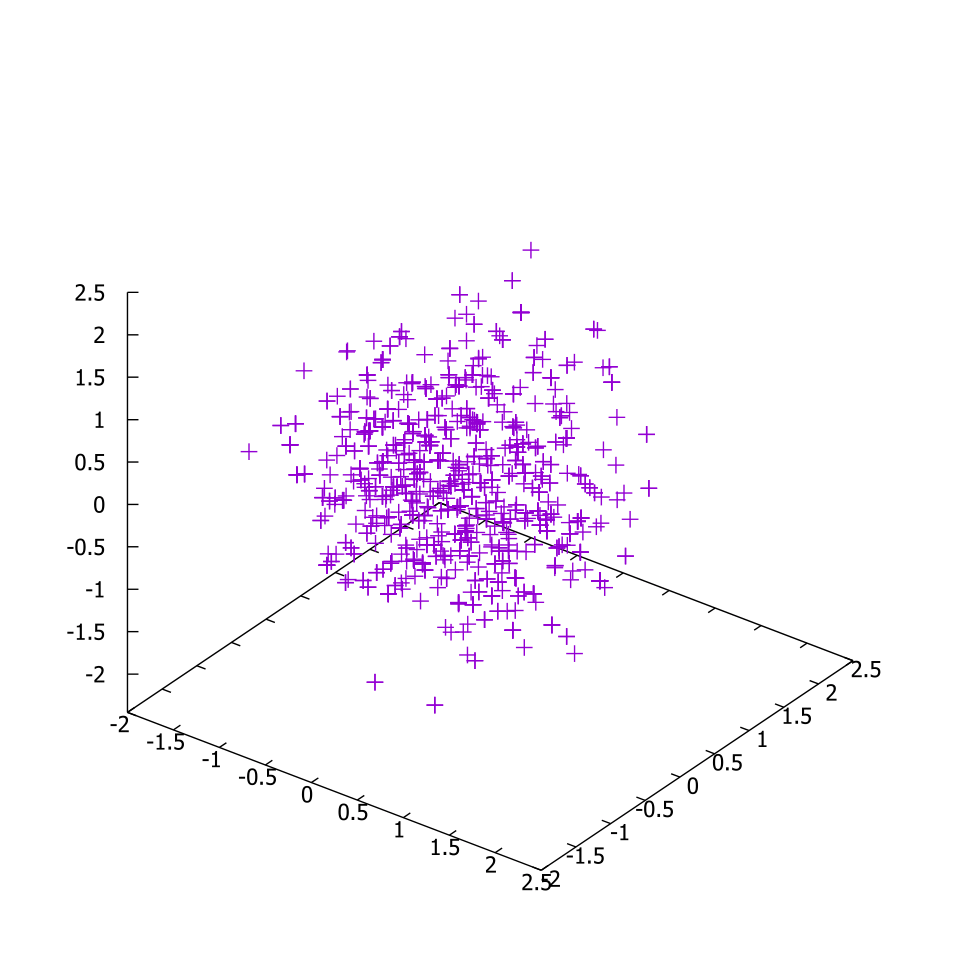
\includegraphics[width=7cm]{gaussian distribution.png}\\
		\caption{타임 함수를 이용하여 난수 설정을 배운 다음 이번에는 조건을 주어 확률을 조정하여서 가우스 분포(정규 분포)를 몬테카를로 시뮬레이션을 이용하여 그려보았다. 조건이 달라지니 아까 의 그림 2와는 다르게 점들이 중심 쪽에 분포해 있는 것을 알 수 있다.} 
		\label{Fig03}
	\end{center}
\end{figure}

\subsection{Simulation of Voter model on a directed network}

본 연구의 선행연구인 정범준 교수 외 2명의 ‘Voter model on a directed network: Role of bidirectional opinion exchanges’에는 3진 트리 모형에서의 레벨 (Level) 수를 변화하면서 전체적인 변화를 확인하였다. 여기서 Level이란 3진 트리의 깊이를 나타내는 변수이다.
본 연구에서는 중심연구를 시행하기 전에 선행연구에서 나온 결과 값들을 확인해 보고자 한다.
우선 각각의 개체는 3진 트리에서 연결되어 있는 개체와만 의사소통이 가능하며 상부개체가 하부개체에 영향을 주는 군대 형 모델이다. 각각의 개체에는  σ(-1또는 1)의 값이 무작위로 들어있는데, 예외적으로 가장 상부에 존재하는 개체에는 반드시 -1을 넣어준다. 1은 옳은 의견, -1은 잘못된 의견을 뜻한다.  임의로 개체 a를 선택하고 개체 a에게 직접적으로 영향을 줄 수 있는 개체(연결된 개체)들 중 임의로 개체 b를 선택한다. 개체 b에 들어 있는 값이 1이면 반드시 개체 a는 1의 값을 가지게 된다. 그러나 만약 개체 b에 들어 있는 값이 -1이면 그와 개체 a는 1-ε의 확률로 -1의 값을 갖게 되고 ε의 확률로 자신 원래의 σ 값을 유지한다. 이 과정을 t번 반복하여 집단 전체의 의견인 σ의 평균 값(m)을 구한다. t 값이 매우 커지면 m이 일정한 값에 수렴하게 된다. 즉, 집단이 의견을 수렴하게 된다.
선행 연구에서 나온 결과와 값들을 확인하기 위하여 본 연구자들은 직접 C++ 언어를 이용하여 코드를 작성 하였고 그에 따라서 직접 여러 가지 결과 값들을 구할 수 있었다.
ε의 값을 0.1로 고정하고 Level 값을 다르게 하면서 그래프 작도 프로그램인 GNUPLOT을 이용하여 그래프를 그려보면 Fig. \ref{Fig04} 와 같은 그래프를 얻을 수 있다.
 
\begin{figure}[t]
 	\begin{center}
 		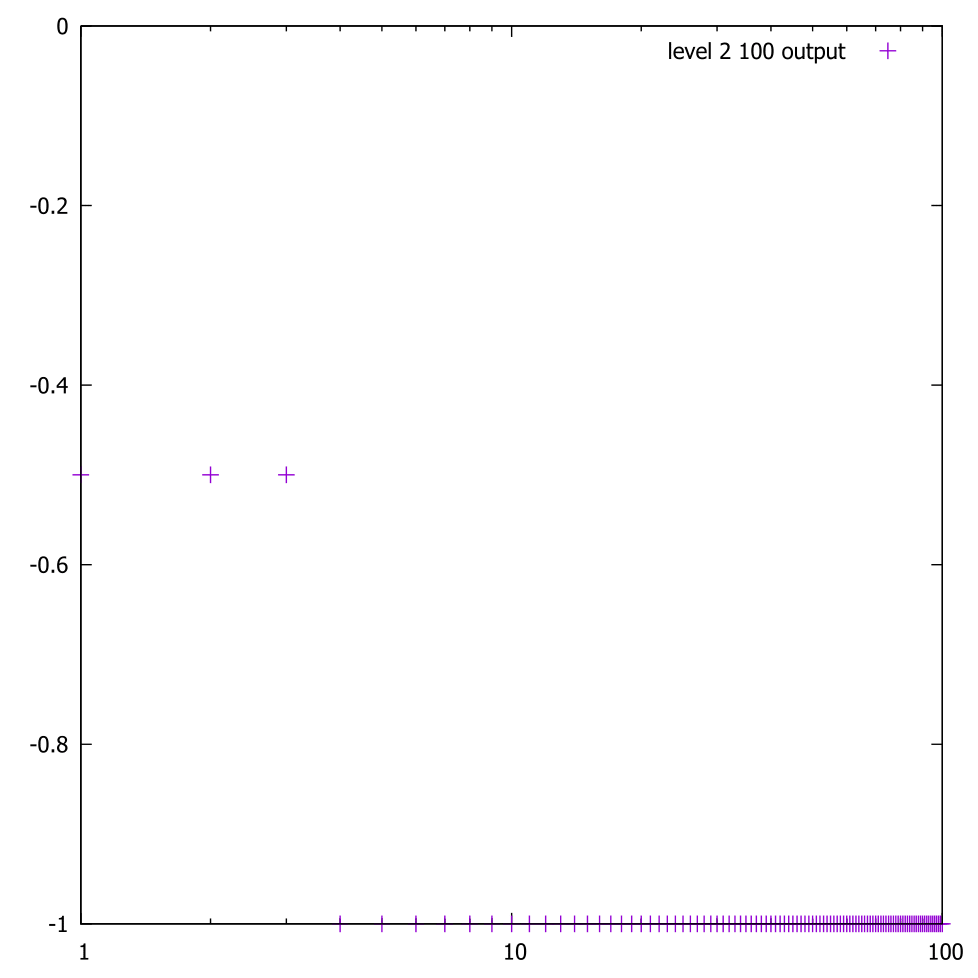
\includegraphics[width=3.5cm]{(a).png}
 		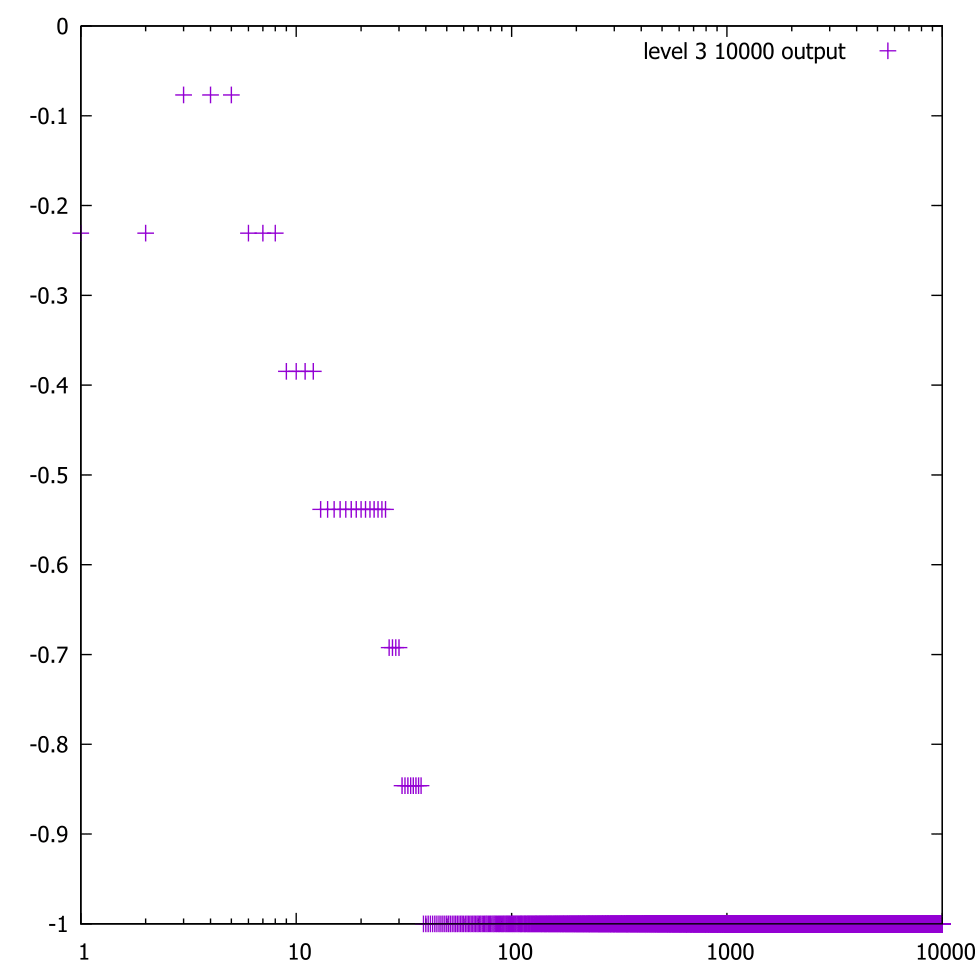
\includegraphics[width=3.5cm]{(b).png}
 		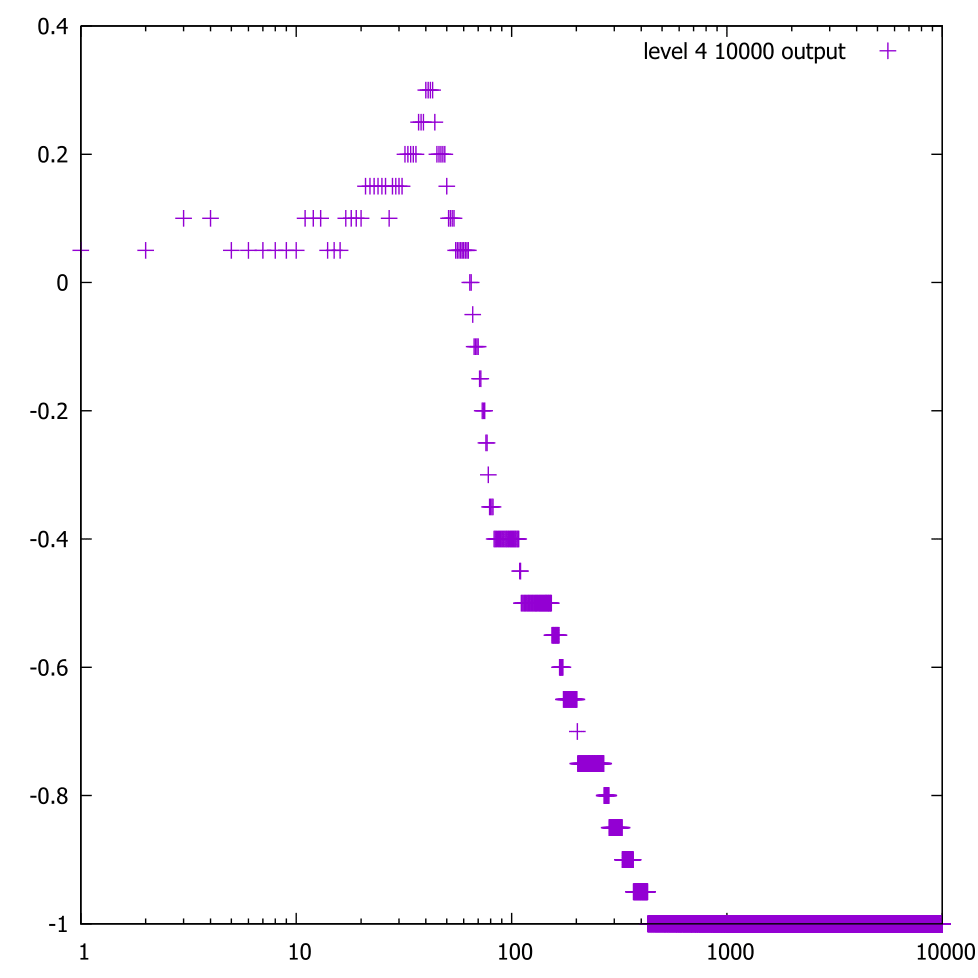
\includegraphics[width=3.5cm]{(c).png}\\
 		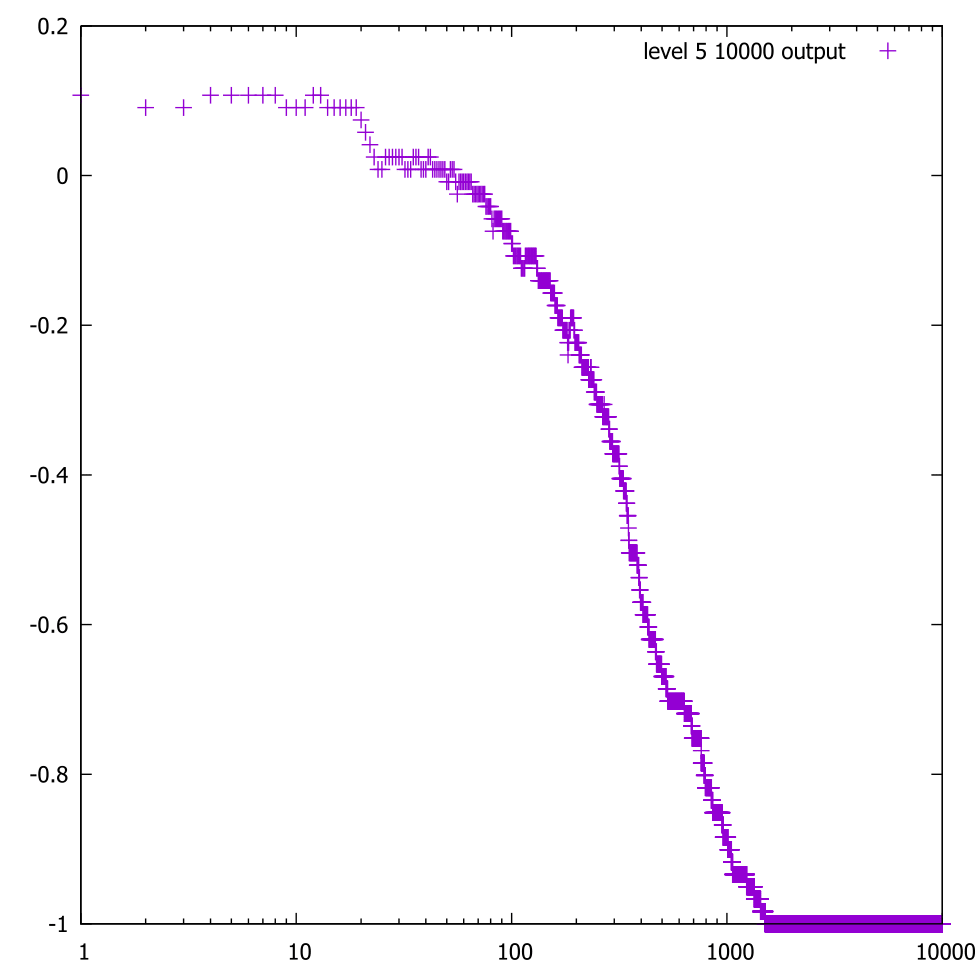
\includegraphics[width=3.5cm]{(d).png}
 		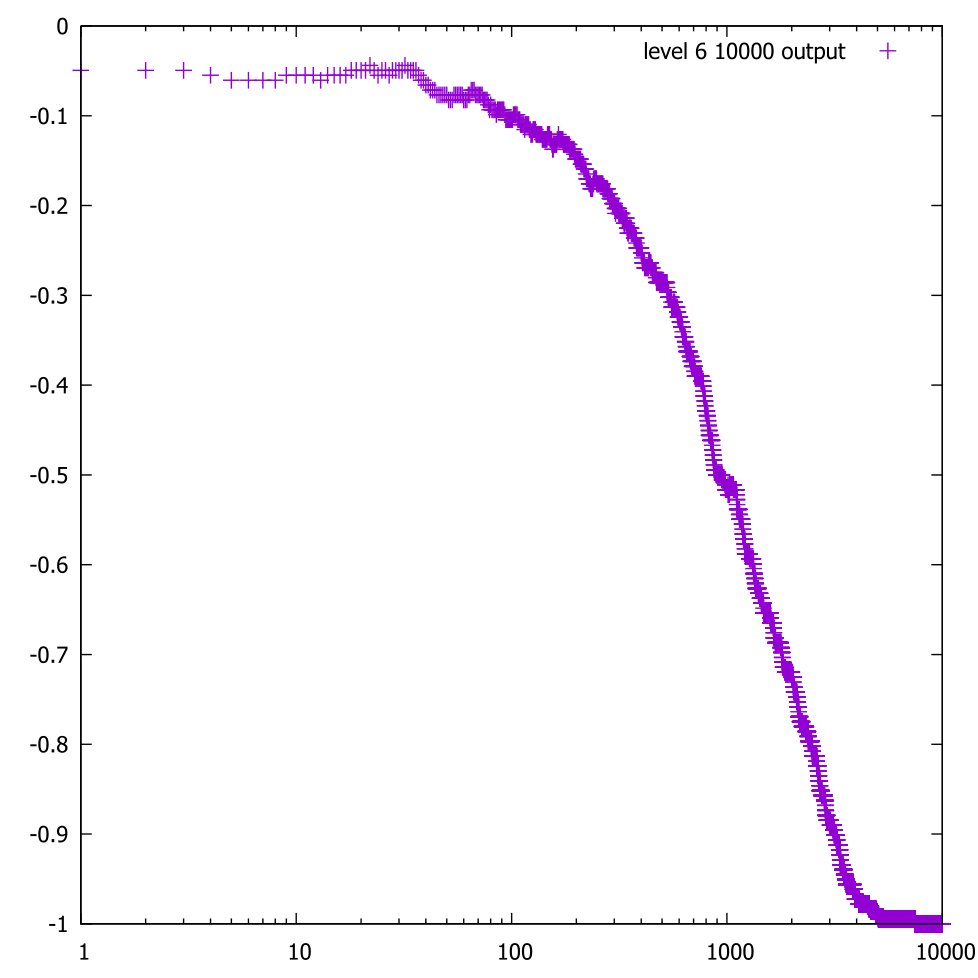
\includegraphics[width=3.5cm]{(e).png}
 		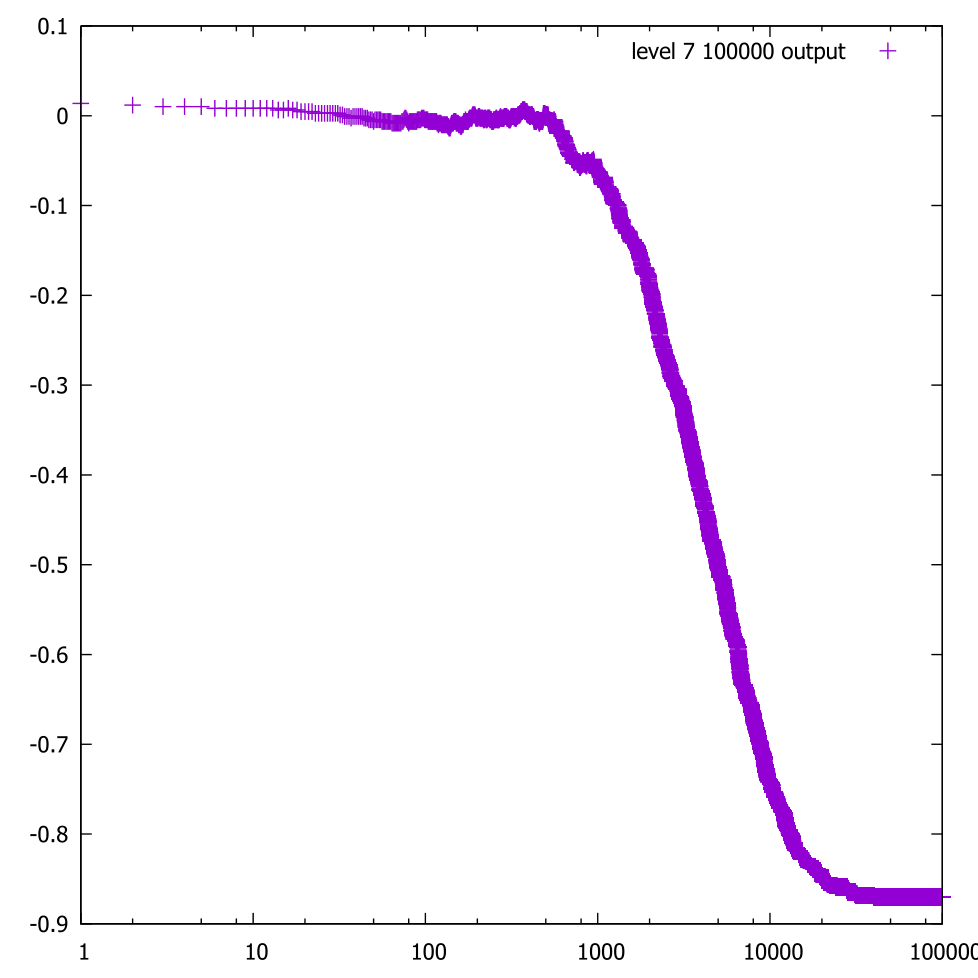
\includegraphics[width=3.5cm]{(f).png}
 		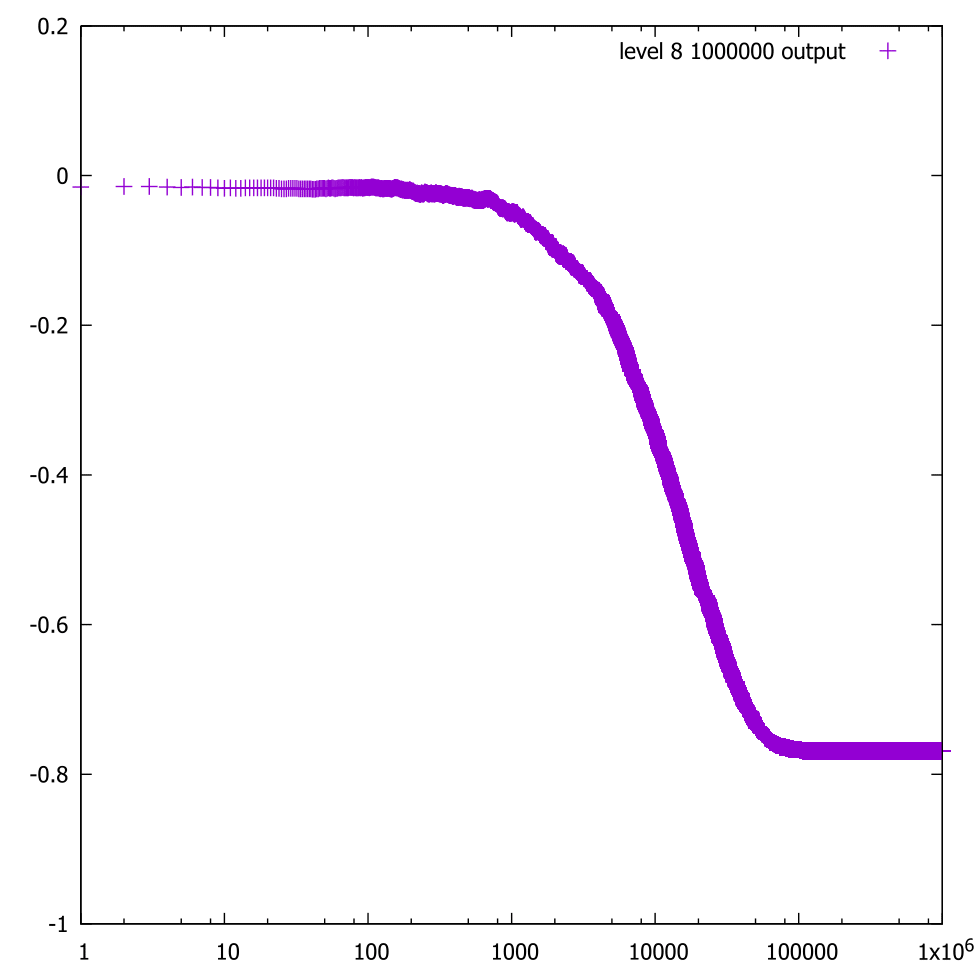
\includegraphics[width=3.5cm]{(g).png}\\
 		\caption{그래프의 x축은 반복된 횟수를 나타내는 변수인 Monte-Carlo time(t)을 나타내고 그래프의 y축은 전체 값들의 평균을 나타내는 변수 m을 나타낸다.} 
 		\label{Fig04}
 	\end{center}
\end{figure}

Graph. a는 Level=2의 그래프인데, m이 급격히 감소하여 Monte-Carlo time이 10이 되기도 전에 -1에 수렴함을 알 수 있다. Graph. b와 Graph. c는 각각 Level=3 일 때의 그래프와 Level=4 일 때의 그래프이다. 두 그래프 모두 Monte-Carlo time이 증가함에 따라 어느 정도 증가하다가 모두 Monte-Carlo time이 1000이 되기 전에 모두 m이 –1로 수렴함을 알 수 있다. 각각 Level 값이 5와 6인 Graph. d와 e 또한 수렴하는 Monte-Carlo time은 이전의 두 그래프보다 더 크지만 이전의 그래프들과 마찬가지로 -1에 수렴한다.  
하지만 Level 값이 7과 8인 경우에는 Graph. f와 g에서 볼 수 있듯이 Monte-Carlo time이 증가하여도 -1에 수렴하지 않고 특정한 값에 m이 수렴한다. 본 연구자들은 이 어느 값에 수렴하는지 알아보기 위하여 실험을 여러 번 하여 수렴하는 의 값의 평균을 구해보았다. 그 결과 Level이 7인 경우 m이 평균적으로 약 -0.868에 값이 수렴하였고 Level이 8인 경우 m이 평균적으로 약 –0.769에 값이 수렴함을 알 수 있었다.
전체적으로 모든 그래프가 m이 -1에 근접한 수에 수렴하는 이유는 초기에 가장 상부 개체에 -1의 값을 대응시켰기 때문이다. 만약 가장 상부 개체에 -1이 아닌 1을 대응시킨다면 m은 1에 수렴한다. 이에 대한 것을 그래프로 그려보면 다음의 Graph. h(Fig. \ref{Fig05})와 같다.\\

\begin{figure}[h]
	\begin{center}
		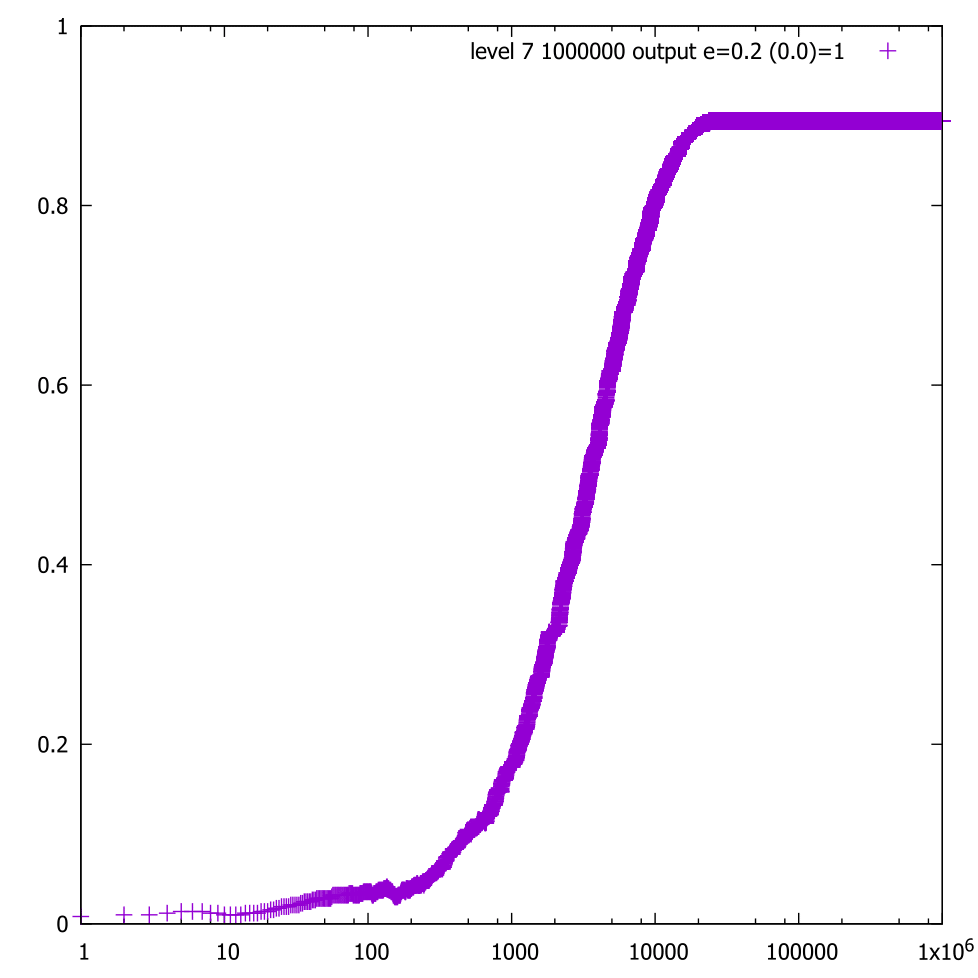
\includegraphics[width=5cm]{(h).png}\\
		\caption{가장 상부 개체에 -1이 아닌 +1을 대응시킨다면 m은 1에 수렴한다.} 
		\label{Fig05}
	\end{center}
\end{figure}

또한 전체적인 변화에 영향을 미치는 Level을 7로 고정시키고 ε의 값을 0.1, 0.2, 0.5 로 변화시켜 보았다. 이때의 그래프를 그려보면 각각 아래의 Graph. f, i, j(Fig. \ref{Fig06})에 대응된다.

\begin{figure}[h]
	\begin{center}
		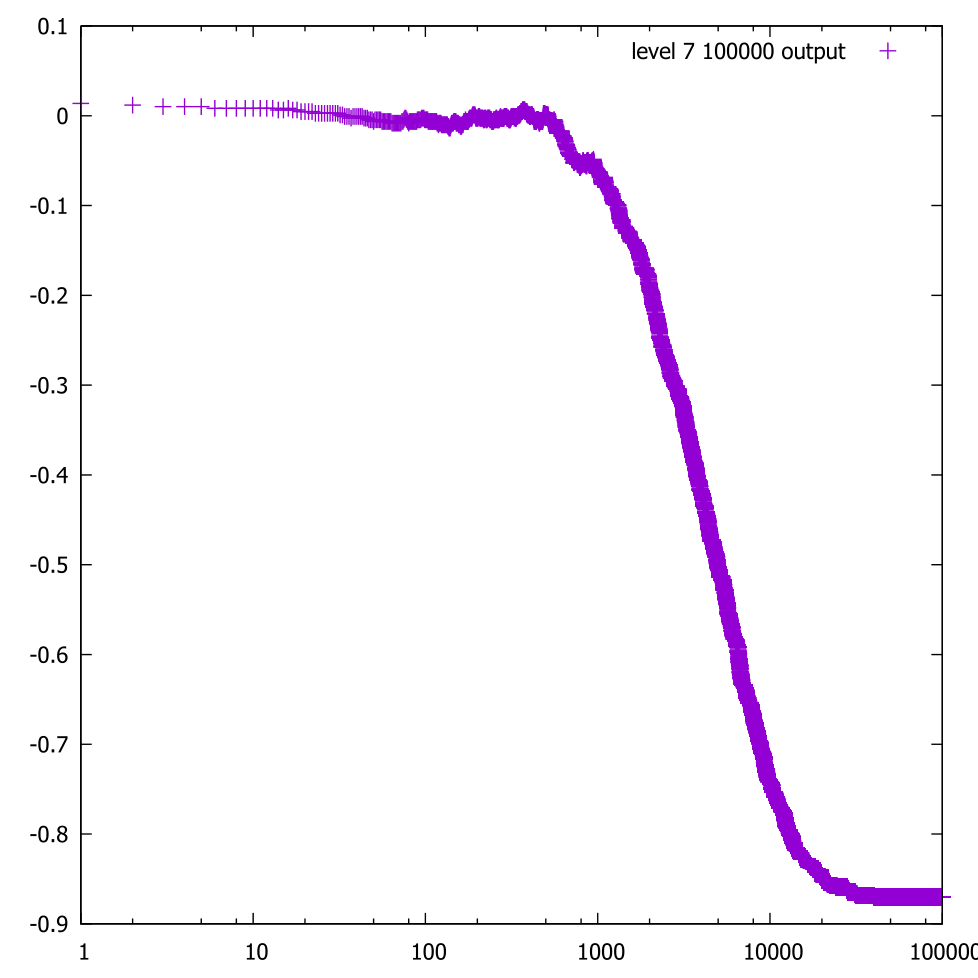
\includegraphics[width=5cm]{(f).png}
		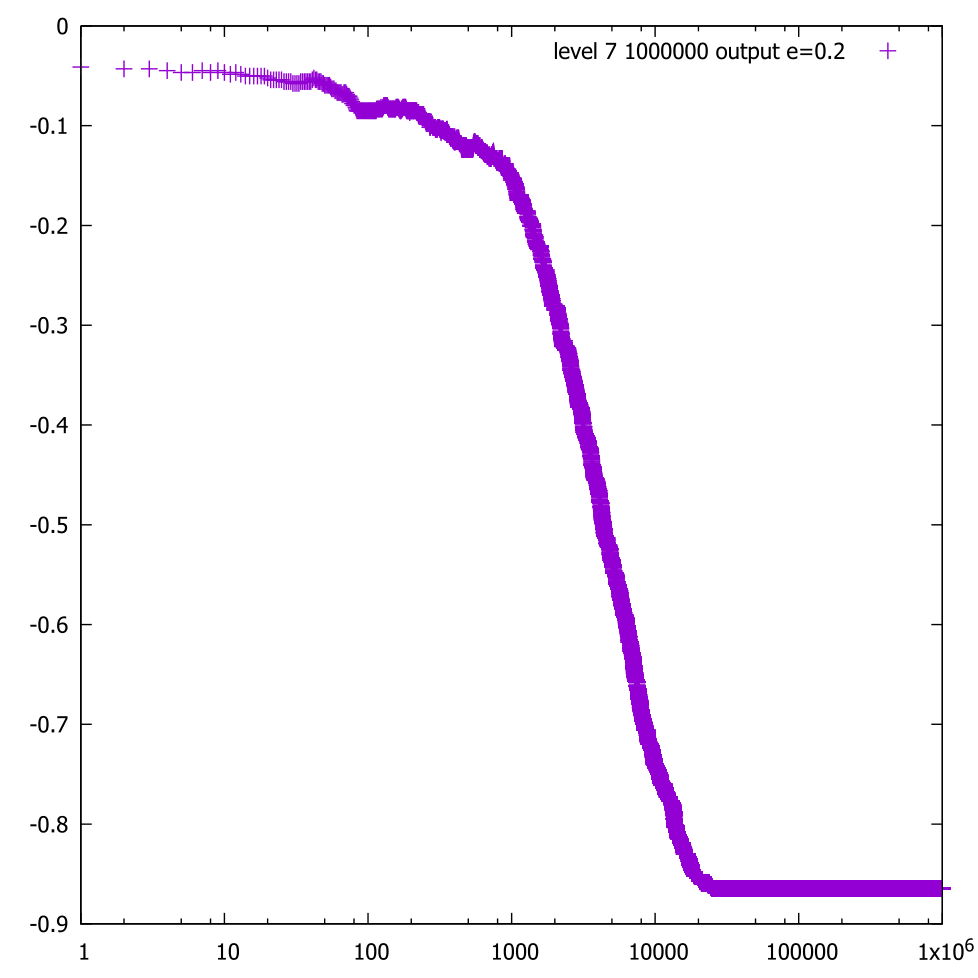
\includegraphics[width=5cm]{(i).png}
		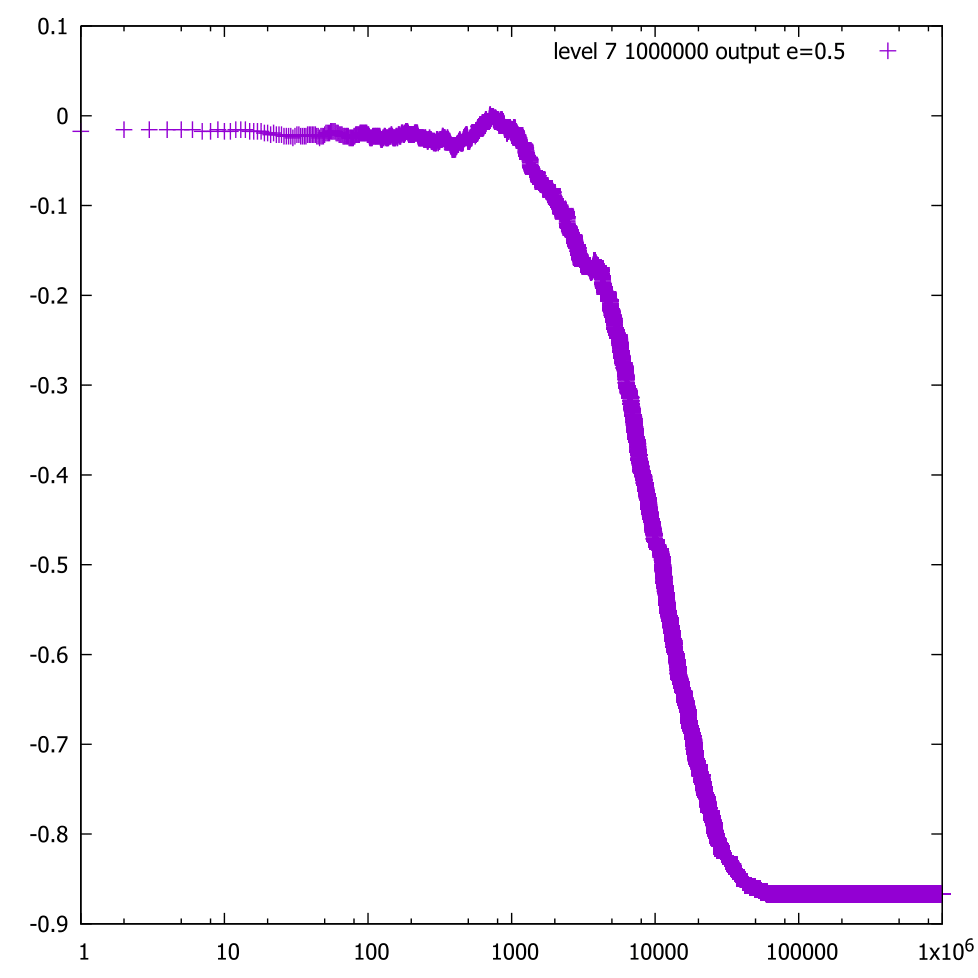
\includegraphics[width=5cm]{(j).png}\\
		\caption{Level을 7로 고정시키고 ε의 값을 0.1, 0.2, 0.5 로 변화시켜 보았다.} 
		\label{Fig06}
	\end{center}
\end{figure}

위 그래프들의 변화에서 알 수 있듯이 ε가 커지면 m이 일정한 값에 수렴하는 Monte-Carlo time이 커진다는 것을 알 수 있다. 이는 ε가 커지면 커질수록 상부개체에 들어있는 값이 -1일 때 하부개체가 -1로 바뀌지 않을 확률이 높아지기 때문이다. 

\section{결론}

본 연구 내용에서 실행한 기존의 몬테카를로 시뮬레이션을 통해 몬테카를로 시뮬레이션을 앞으로의 연구에 사용할 수 있게 되었다. 또한, p=0인 군대 형 3진 트리 모형에서 맨 위 개체가 -1의 값을 가지면 집단 전체가 -1의 값을 가지게 되는 결과를 통해 군대형 구조에서 최고 권위자가 잘못된 결정을 하면 집단 전체가 빠른 시간안에 잘못된 결론을 낸다.
본래 선행연구\cite{Han10}에서는 단순히 군대 형 구조가 아닌 민주적인 정도를 나타내는 변수인 p를 0이상 1이하의 범위 내에서 설정하여(p의 값이 1에 가까울수록 민주적이다) ‘민주적인인 구조가 더 이상적인 결론을 낼 수 있다’라는 것을 통계역학적으로 증명하였다. 그러나 본 연구자들은 아직 그에 대한 연구를 진행하고 있고 또한 아직 발전시켜야 할 여지가 많다. 
또한 본래 계획했던 메인 주제인 ‘각각의 개체에 가중치(권위)를 부여하고 가중치의 차이에 따른 확률의 변화를 생각한 모델’ 또한 아직 구현 중에 있다. 앞으로 시간에는 이에 대한 연구에 집중할 계획이다. 


%%
%% 영어 보고서 참고문헌 시작
%% Refences
%%
\begin{thebibliography}{99}

\bibitem{Stauffer06} D. Stauffer, S. Moss de Oliveira, P. de Oliveira, and J. Martins, ``Biology, sociology, geology by computational
physicists s'', Elsevier, Amsterdam, {\bf 10000}, 10000 (2006).
\bibitem{Stauffer08} D. Stauffer,and S. Solomon, ``Applications of Physics and Mathematics to Social Science'', J. Geophys. Res., {\bf 79}, 2803 (1974).
\bibitem{Hegselmann02} Rainer Hegselmann, and Ulrich Krause, ``Opinion dynamics and bounded confidence models, analysis, and simulation'', Journal of Artifical Societies and Social Simulation, {\bf 5}, no.3 (2002).
\bibitem{Han10} Sung-Guk Han, Jaegon Um, and Beom Jun Kim ``Voter model on a directed network: Role of bidirectional opinion exchanges'', Phys. Rev. E, {\bf 81}, 057103 (2010).
\bibitem{Frachebourg96} L. Frachebourg and P. L. Krapivsky, ``Exact Results for Kinetics of Catalytic Reactions'', Phys. Rev. E, {\bf 53}, R3009 (1996).
\bibitem{Castellano09} Claudio Castellano, Santo Fortunato, and Vittorio Loreto, ``Statistical physics of social dynamics'', Rev. Mod. Phys, {\bf 81}, 591 (2009).

\end{thebibliography}

%%
%% 한글참고문헌 시작
%% Refences
%%
%\begin{thebibliographykor}{99}
%
%\bibitem{Iijima91} 김익수, 원색 한국 어류도감, 아카데미, 1993, pp.33-65
%
%\bibitem{Dresselhaus96} IAL L. Pepper, Pollution Science, Academic Press, 1996, pp.145-188
%
%\bibitem{Saito98}이은웅, 김일중,``2상 8극형 HB형 리니어 펄스모터의 자속 분포와 정특성 해석'', 대한전기학회 논문지, 제42권 9호, pp.9-18, 1993.
%
%\bibitem{Makarova01} G. Taylor et al., ``Adaptive regulation of nonlinear systems with unmodeled dynamics'', IEEE Trans. Automat. Contr., Vol. 34, pp. 997-998, 1994.
%
%\end{thebibliographykor}
\end{document}
